\section{Aufbau}
Bestehend aus grzundsätzlich drei Hauptteilen setzt sich das Experiment wie folgt zusammen:
\begin{itemize}
    \item{Kuper-Röntgenröhre}
     \item{LiF-Kristall}
     \item{Geiger-Müller-Zählrohr}
     \item{Schlitzblende}
\end{itemize}
Die Röntgenröhre behinhaltet außerdem die Elektronik um das elektrische Feld zu erzeugen und die Elektronen zu beschleunigen.
Zur Auswertung wird ein Rechner benutzt. Dieser ist in der Lage, durch passende Programmauswahl, genau auf das Problem zugeschnitten zu messen. 
Hier lassen sich mehrere Paramter einstellen. 
\begin{itemize}
     \item{Kristallwinkel}
        %\intertext{}
     \item{Integrationszeit}
        %\intertext{}
     \item{Messart}
        %\intertext{sollte auf $Spektren$ gestellt sein. (Einzige relevante Messung) }
     \item{Drehmodus}
        %\intertext{}
\end{itemize}
Die Messart sollte im Verlauf immmer auf Spektren stehen, da das der einzige relevante Messwert ist. Anbei sind außerdem mehrere Blenden für die Absorbationsmessung.

\begin{figure}
    \centering
    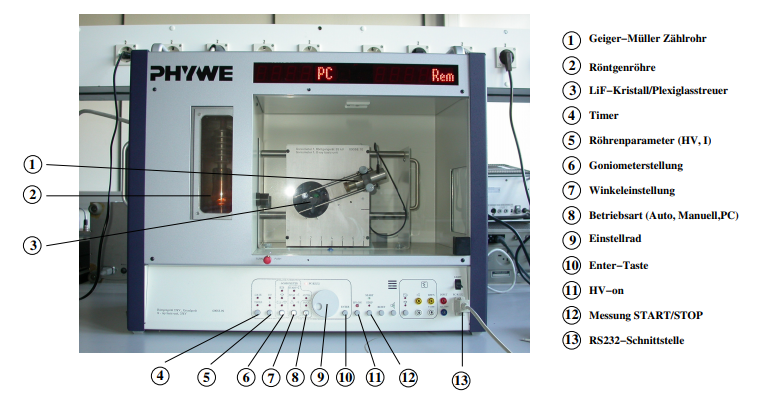
\includegraphics[width=\textwidth]{bilder/Screenshot 2021-01-29 104244.png}
    \caption{Rechner. Messgerät und Konfigurator \cite{skript}. } 
    \label{fig:Rechner}
\end{figure}